\documentclass[11pt]{article}

% Include basic packages
\usepackage{setspace}\doublespacing
\usepackage[usenames,dvipsnames]{xcolor} % more color options by name
\usepackage{amsmath,amsfonts,amssymb,fleqn,graphicx,mathtools,color} % math, figures
\setlength{\abovecaptionskip}{10pt} % Chosen fairly arbitrarily
\usepackage[font=small,labelfont=bf]{caption}
\usepackage{auto-pst-pdf} % for ps files
\usepackage{array,booktabs,ragged2e}
\newcolumntype{R}[1]{>{\RaggedLeft\arraybackslash}p{#1}} % allow right justified cells in table


% Set margin formatting
\usepackage[headheight=65pt]{geometry}
\geometry{
  top=1 in,
  inner=0.9 in,
  outer=0.9 in,
  bottom=1 in,
  headheight=3ex,
  headsep=6ex,
}

% Set header formatting
\usepackage{fancyhdr}
\pagestyle{fancy}
\fancyfoot{}
\chead{\assgn}
\rhead{Page \thepage}
\renewcommand{\headrulewidth}{1pt}

% Allow links within document
\usepackage{hyperref}
\usepackage{cleveref}
\usepackage{pgfplots}
\hypersetup{colorlinks=true,linkcolor=Black,urlcolor=blue}

% Enable code insertion from local file
\usepackage{listings}
\usepackage{csvsimple}

% Define some parameters for better formatting of inserted code
\lstset{
    basicstyle=\fontsize{9}{7}\ttfamily, % typewriter font family
    columns=flexible,
    keywordstyle=\color{blue}\ttfamily, % make keywords blue
    stringstyle=\color{red}\ttfamily, % make strings red
    breaklines=true, % wrap long lines
    commentstyle=\color{ForestGreen}\ttfamily % more readable than default color
}

\lstdefinestyle{pythonstyle}{
    language=Python,
    basicstyle=\ttfamily\small,
    keywordstyle=\color{blue}\bfseries,
    stringstyle=\color{orange},
    commentstyle=\color{green!50!black},
    numbers=left,
    numberstyle=\tiny\color{gray},
    stepnumber=1,
    numbersep=8pt,
    backgroundcolor=\color{gray!10},
    frame=single,
    breaklines=true,
    showstringspaces=false,
    tabsize=4
}

\lstdefinestyle{cstyle}{
    language=C,
    basicstyle=\ttfamily\small,
    keywordstyle=\color{blue}\bfseries,
    stringstyle=\color{orange},
    commentstyle=\color{green!50!black},
    numbers=left,
    numberstyle=\tiny\color{gray},
    stepnumber=1,
    numbersep=8pt,
    backgroundcolor=\color{gray!10},
    frame=single,
    breaklines=true,
    showstringspaces=false,
    tabsize=4
}

\newif\ifcode % define toggle for code insertion
\codetrue % toggle by commenting/uncommenting

% Set personal info, class, assignment
\def \fnamea{David}
\def \lnamea{Ran}
\def \class{CS 553}
\def \hwnum{4} % Homework number
\def \assgn{Homework Report \hwnum}

% Begin document
\begin{document}

% Author, Title, Abstract, TOC
\title{\class: \assgn}
\author{\fnamea\ \lnamea}
\date{\today}
\maketitle
\tableofcontents

% TEMPLATE FOR FIGURE IF NEEDED
% \begin{figure}[htp]
%     \centering
%     \includegraphics[width=15cm]{TBD.png}
%     \caption{SOME CAPTION}
%     \label{fig:tbd}
% \end{figure}



\newpage
%%%%%%%%%%%%%%%%%%%%%%%%%%%%%%%%%%%%%%%%%%%%%%%%%%%%%%%%%%%%
\section{Introduction}

This assignment asks us to optimize a PolyBench kernel under a function-body-only constraint, using the profiling and measurement tooling we built up over the semester. The target was \texttt{datamining/correlation}: compute a Pearson correlation matrix on $N$ observations of $M$ variables.

The approach taken here departs from a traditional solo workflow. Rather than writing the C and Python directly, I directed an AI coding assistant (Claude) to instrument the kernel, run the experiment-helper studies, and implement candidate optimizations under my judgment. The intent was to test whether the existing tool chain --- correctness gate, runtime study, hardware-counter study, trimmed-mean analysis --- could carry an AI collaborator through a non-trivial optimization without me writing the code by hand. The measured result is a \textbf{44$\times$ whole-kernel speedup at $N{=}2048$, $-O3$}, bit-identical (within $10^{-6}$ tolerance) to the upstream output. The collaboration process is documented separately in Section~\ref{sec:genai}.


%%%%%%%%%%%%%%%%%%%%%%%%%%%%%%%%%%%%%%%%%%%%%%%%%%%%%%%%%%%%
\section{Experimental Setup}

All experiments ran on the course evaluation machine, an Intel Xeon E-2278G (Coffee Lake, 8 cores, 3.4--5.0 GHz, AVX2, no AVX-512). Caches are 32~KB L1d/core, 256~KB L2/core, and 16~MB shared L3; main memory is dual-channel DDR4-2666. PAPI 6.0.0.0 exposes ten hardware counters with no multiplexing required, so all derived metrics in this report come from a single counted run per configuration.

The architectural DP peak per core is $2~\text{FMA} \times 4~\text{lanes} \times 2~\text{ops} = 16~\text{FLOPs/cycle}$, so any FLOPs/cycle figures should be read against that ceiling. Compilation used \texttt{gcc} with \texttt{-O2} and \texttt{-O3}; \texttt{-O3} is the headline figure because both auto-vectorization and the explicit register-blocked region~4 require it to fire.

The experiment driver (\texttt{experiment\_helper.py}) sweeps $\text{Size} \times \text{Opt\_Level} \times \text{TIME\_REGION}$ in a round-robin order with 10 runs per configuration; reported numbers are trimmed means (min and max dropped). Square sizes $N \in \{128, 512, 2048\}$ span the L1, L2/L3-fit, and DRAM-bound regimes respectively.


%%%%%%%%%%%%%%%%%%%%%%%%%%%%%%%%%%%%%%%%%%%%%%%%%%%%%%%%%%%%
\section{Profiling and Measurement Strategy}

\subsection{Region-level timing}

The upstream kernel has four loop nests: (1)~per-column mean, (2)~per-column stddev, (3)~per-element centering, and (4)~the $O(M^2 N)$ correlation matrix. To time each one independently without disturbing the compiler's view of the code, \texttt{correlation.localized.c} wraps each region with \texttt{\#if TIME\_REGION == r} guards around the existing \texttt{polybench\_start\_instruments} / \texttt{polybench\_stop\_instruments} calls. A separate compile selects each region; the whole kernel ($\texttt{TIME\_REGION=0}$) is the un-modified baseline timing for sanity-checking the parts against the whole. The optimized variant adds \texttt{TIME\_REGION=5} (transpose) and \texttt{TIME\_REGION=6} (fused stats+center).

This guards-only approach was chosen over a function-based refactor specifically to preserve the compiler's inlining, aliasing, and register-allocation decisions. The data flow is unchanged across all values of \texttt{TIME\_REGION}, so the final \texttt{corr} matrix is bit-identical regardless of which region is being timed.

\subsection{Hardware counter set}

The ten available counters are budgeted as in Table~\ref{tab:counters}. From these, nine derived metrics are computed; the most load-bearing for this kernel are:

\begin{itemize}
\setlength\itemsep{0pt}
  \item \textbf{FLOPs/cycle} $= \texttt{DP\_OPS}/\texttt{TOT\_CYC}$ --- against the architectural peak of 16.
  \item \textbf{Arithmetic intensity} (AI) $= \texttt{DP\_OPS}/(\texttt{L3\_TCM} \times 64)$ --- DRAM-level FLOPs per byte; the roofline x-axis.
  \item \textbf{DP\_per\_vec} $= \texttt{DP\_OPS}/\texttt{VEC\_DP}$ --- effective lane utilization; AVX2 FMA ideal is 8.
  \item \textbf{\%L3m, \%Stall} --- where the cycles go when the pipe is empty.
\end{itemize}

\begin{table}[htp]
\centering
\small
\begin{tabular}{l l}
\toprule
Counter & Used in \\
\midrule
\texttt{PAPI\_DP\_OPS}    & FLOPs/cycle, AI, DP\_per\_vec \\
\texttt{PAPI\_L3\_TCM}    & AI, \%L3m \\
\texttt{PAPI\_TOT\_CYC}   & FLOPs/cycle, IPC, vIPC, \%Stall denom. \\
\texttt{PAPI\_TOT\_INS}   & IPC \\
\texttt{PAPI\_LST\_INS}   & \%L1m denom. \\
\texttt{PAPI\_L1\_DCM}    & \%L1m, \%L2m denom. \\
\texttt{PAPI\_L2\_TCM}    & \%L2m \\
\texttt{PAPI\_L3\_TCA}    & \%L3m denom. \\
\texttt{PAPI\_RES\_STL}   & \%Stall \\
\texttt{PAPI\_VEC\_DP}    & vIPC, DP\_per\_vec \\
\bottomrule
\end{tabular}
\caption{Counter budget. Ten counters available, ten used --- no multiplexing.}
\label{tab:counters}
\end{table}

\subsection{Correctness gate}

Every change passes \texttt{check\_correctness.py opt} before measurement: rebuild with \texttt{-DTIME\_REGION=0 -DPOLYBENCH\_DUMP\_ARRAYS} and diff the dumped \texttt{corr} matrix element-wise against the upstream reference at $10^{-6}$ tolerance. The opt variant is currently bit-identical to upstream (max diff $0.000$e$+00$).


%%%%%%%%%%%%%%%%%%%%%%%%%%%%%%%%%%%%%%%%%%%%%%%%%%%%%%%%%%%%
\section{Optimization Strategy}

\subsection{Bottleneck}

\texttt{data} is row-major $[N][M]$. Three of the four regions read it column-walk (stride $M$), region~4 reads it twice column-walk inside an $O(M^2 \cdot N)$ loop. The baseline is therefore both (a)~unvectorizable on the inner loop and (b)~cache-hostile, with both effects getting worse as $N$ grows.

\subsection{Applied transformations}

All three live in \texttt{correlation.opt.c}; the math is unchanged from upstream.

\paragraph{1. In-kernel blocked transpose.} Allocate a scratch \texttt{dataT[M][N]} at the top of \texttt{kernel\_correlation} and fill it via a 16$\times$16 blocked transpose. All four regions then read \texttt{dataT} instead of \texttt{data}, making every inner-loop access unit-stride. Cost is one extra $O(M \cdot N)$ pass plus $M{\cdot}N{\cdot}8$ bytes of scratch; this is the foundation that everything else builds on. New timed region: \texttt{TIME\_REGION=5}.

\paragraph{2. Column-at-a-time fusion of stats + center.} The original kernel sweeps \texttt{dataT} three separate times (mean, stddev, center), each from DRAM at $N{=}2048$ since \texttt{dataT} is $\sim$32~MB (larger than L3). The optimized variant fuses the three outer-$j$ loops, doing three inner passes per column. Each column is $\sim$16~KB at $N{=}2048$, half of L1, so it stays L1-resident across the three passes. DRAM traffic for the stats+center bundle drops from $\sim$4$M N \cdot 8$ to $\sim$2$M N \cdot 8$ bytes. The original two-pass variance is preserved (the single-pass $\text{Var}(X) = E[X^2] - E[X]^2$ identity was considered and rejected for catastrophic-cancellation risk). Fused region: \texttt{TIME\_REGION=6}.

\paragraph{3. Register-block region 4 with backward $j$.} After the transpose, region~4's inner $k$-loop is already unit-stride and vectorizable. Two further changes squeeze it: (a)~register-block four anchor rows simultaneously (\texttt{CORR\_BI=4}) so one load of \texttt{dataT[j][k]} feeds four independent FMA accumulators per iteration, keeping both FMA ports busy; (b)~iterate $j$ backward within each $i$-tile so the last row used at the end of one tile is the smallest, leaving it hot in L1 at the next tile boundary. Triangular fringe and a tail loop handle the cleanup cases.

\subsection{Rejected ideas}

The most consequential rejection was single-pass variance (above). Also considered and dropped: changing the storage layout of \texttt{data} (would have made the transpose unnecessary --- ruled out by the function-body constraint), $k$-axis tiling of region~4 (spot checks indicated the register-blocked version is already compute-bound), and software prefetch (the hardware prefetcher already saturates the unit-stride streams).


%%%%%%%%%%%%%%%%%%%%%%%%%%%%%%%%%%%%%%%%%%%%%%%%%%%%%%%%%%%%
\section{Results}

\subsection{Whole-kernel speedup}

\begin{table}[htp]
\centering
\small
\begin{tabular}{r r r r r r}
\toprule
Size & Opt level & Baseline (ms) & Opt (ms) & Speedup \\
\midrule
128  & -O2 &      1.06 &     0.41 & 2.60$\times$  \\
512  & -O2 &    176.20 &    18.66 & 9.44$\times$  \\
2048 & -O2 &  46204.95 &  1225.57 & \textbf{37.70$\times$} \\
\midrule
128  & -O3 &      1.10 &     0.32 & 3.46$\times$  \\
512  & -O3 &    175.82 &    16.75 & 10.50$\times$ \\
2048 & -O3 &  46253.49 &  1048.70 & \textbf{44.11$\times$} \\
\bottomrule
\end{tabular}
\caption{Whole-kernel (\texttt{TIME\_REGION=0}) runtime, trimmed mean of 10 runs. Speedup grows with $N$ because region~4 is $O(M^2 N)$ and its baseline access pattern degrades faster than the work increases.}
\label{tab:speedup}
\end{table}

\begin{figure}[htp]
    \centering
    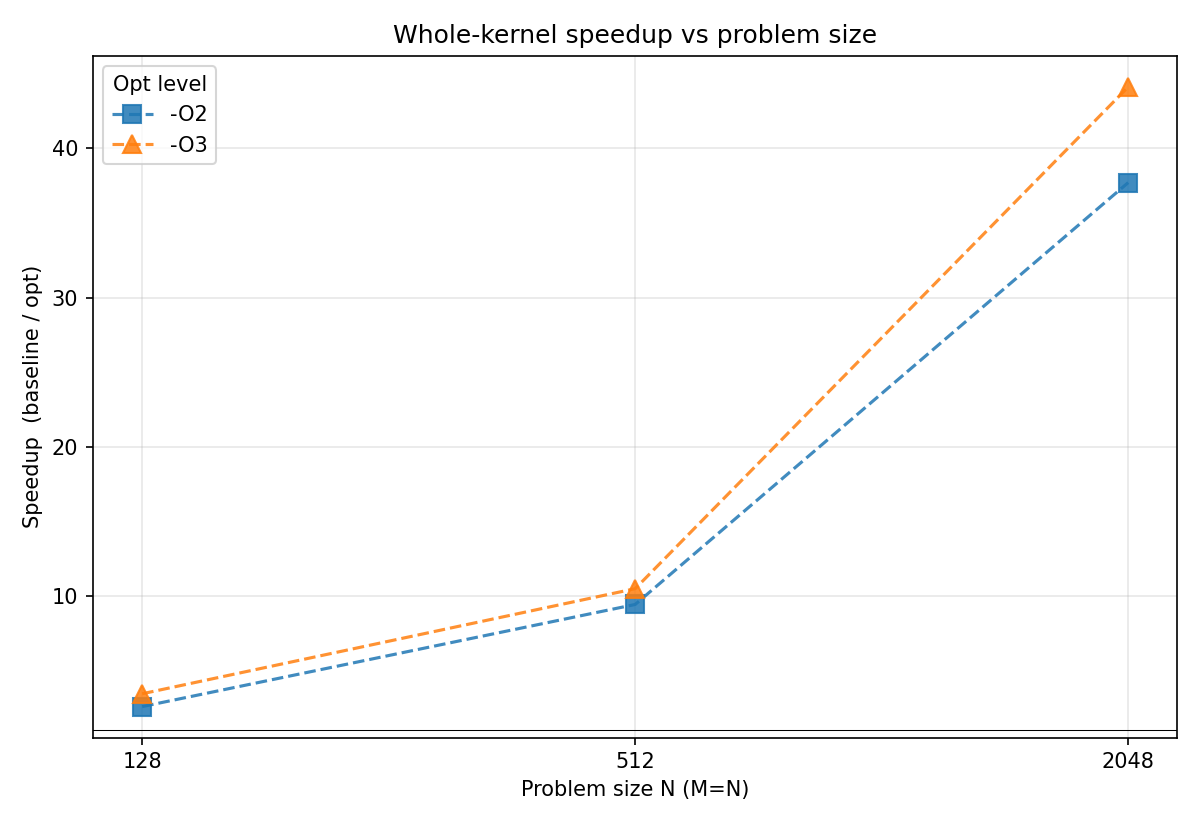
\includegraphics[width=13cm]{../results/speedup_vs_size.png}
    \caption{Whole-kernel speedup vs.\ problem size. Both opt levels scale super-linearly with $N$.}
    \label{fig:speedup}
\end{figure}

\subsection{Region breakdown}

Table~\ref{tab:breakdown} and Figure~\ref{fig:breakdown} decompose the runtime at $-O3$. Region~4 (correlation matrix) is overwhelmingly the dominant cost in the baseline --- 99.9\% of wall time at $N{=}2048$ --- and remains dominant in the opt variant, but is now small enough that the transpose and fused stats+center are visible contributors.

\begin{table}[htp]
\centering
\small
\begin{tabular}{r | r r r r r | r r r r}
\toprule
       & \multicolumn{5}{c|}{Baseline regions (ms)} & \multicolumn{4}{c}{Opt regions (ms)} \\
Size & R1 & R2 & R3 & R4 & total & R5 (xpose) & R6 (stats+ctr) & R4 & total \\
\midrule
128  & 0.01 &  0.01 &  0.01 &     0.96 &     0.99 &  0.03 &  0.03 &    0.27 &    0.33 \\
512  & 0.17 &  0.32 &  0.11 &   176.96 &   177.56 &  0.95 &  0.54 &   15.43 &   16.91 \\
2048 & 12.98 & 22.58 & 2.36 & 46247.80 & 46285.73 & 15.28 & 8.52 & 1024.43 & 1048.24 \\
\bottomrule
\end{tabular}
\caption{Per-region runtime at $-O3$, trimmed mean (ms). R4 baseline$\rightarrow$opt at $N{=}2048$ is 46247.80~ms $\rightarrow$ 1024.43~ms, a 45$\times$ reduction.}
\label{tab:breakdown}
\end{table}

\begin{figure}[htp]
    \centering
    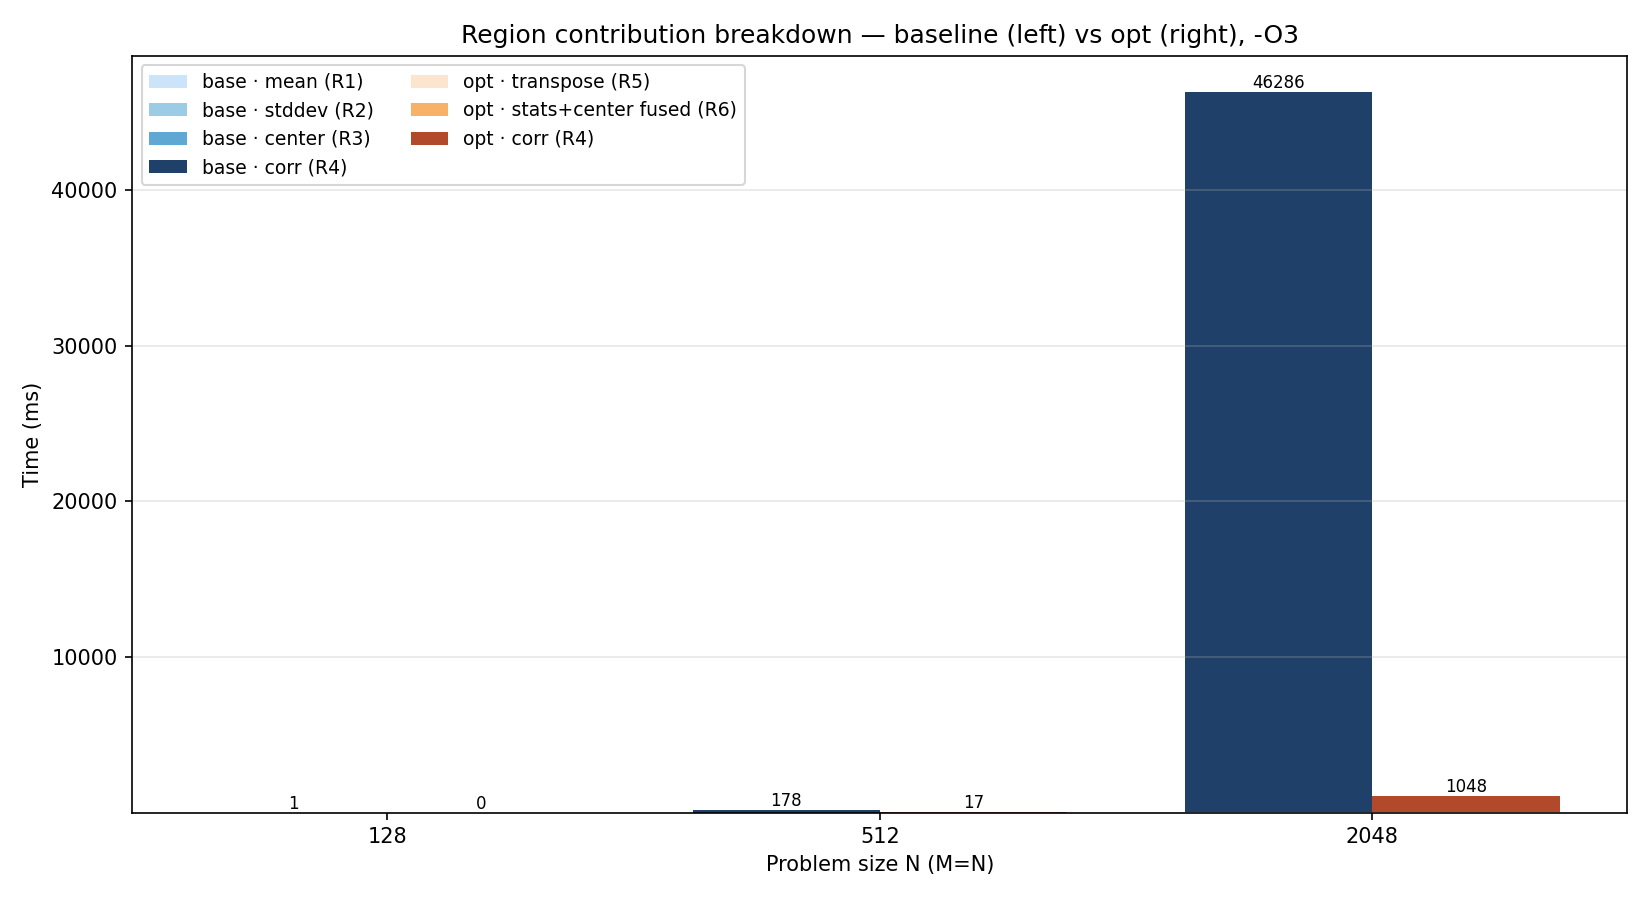
\includegraphics[width=14cm]{../results/breakdown.png}
    \caption{Stacked-bar breakdown of region contributions at $-O3$. Baseline (left bar) is dominated by R4; opt (right bar) has all three regions visible.}
    \label{fig:breakdown}
\end{figure}

\subsection{Hardware counter comparison: region 4 at $-O3$}

Table~\ref{tab:hwmetrics} shows where the speedup comes from at the microarchitecture level.

\begin{table}[htp]
\centering
\small
\begin{tabular}{r | r r | r r | r r | r r}
\toprule
       & \multicolumn{2}{c|}{FLOPs/cycle} & \multicolumn{2}{c|}{DP\_per\_vec} & \multicolumn{2}{c|}{\%L3m} & \multicolumn{2}{c}{\%Stall} \\
Size & base & opt & base & opt & base & opt & base & opt \\
\midrule
128  & 0.41 & 1.89 & 1.00 & 1.33 &  0.0 &  0.0 & 57.95 & 21.45 \\
512  & 0.17 & 1.91 & 1.00 & 1.33 &  0.0 &  0.0 & 80.00 & 22.04 \\
2048 & 0.04 & 1.75 & 1.00 & 1.33 & 78.65 & 27.58 & 95.26 & 29.18 \\
\bottomrule
\end{tabular}
\caption{Region 4 hardware metrics, baseline vs.\ opt, $-O3$. The baseline degrades sharply with size (FLOPs/cycle drops from 0.41 to 0.04, \%Stall climbs to 95\%); the opt variant is stable across sizes. \texttt{DP\_per\_vec} going from 1.0 to 1.33 confirms the compiler emits vector instructions on the opt version that it could not on the strided baseline.}
\label{tab:hwmetrics}
\end{table}

The picture is consistent: the baseline at $N{=}2048$ is DRAM-bound and stalled (\%L3m 79\%, \%Stall 95\%, FLOPs/cycle 0.04 --- about 1/400 of the architectural peak). The opt variant cuts L3 miss rate to 28\%, stalls to 29\%, and reaches 1.75 FLOPs/cycle (about 11\% of peak). The remaining gap to peak is consistent with the inner loop being limited by load throughput and the 1.33 DP\_per\_vec figure suggests the compiler is still emitting some scalar/partial-width instructions in the fringe; further headroom likely exists but the work to extract it is no longer cheap.

\subsection{Summary}

The optimized kernel is bit-identical to upstream output and runs 44$\times$ faster at $N{=}2048$, $-O3$. The cost is $\sim$$N{\cdot}M{\cdot}8$ bytes of scratch heap and a few hundred lines of in-kernel code. The dominant win comes from the transpose (regions 1, 2, 4 all become unit-stride), with column-at-a-time fusion contributing a $\sim$2$\times$ reduction in stats+center DRAM traffic and the register-block + backward-$j$ contributing $\sim$3$\times$ on region~4 on top of the transpose.


%%%%%%%%%%%%%%%%%%%%%%%%%%%%%%%%%%%%%%%%%%%%%%%%%%%%%%%%%%%%
\section{Discussion on GenAI Usage}
\label{sec:genai}

This project was carried out as an explicit human/AI collaboration. The AI (Claude) wrote all C and Python code in the repository; I (the human) chose the direction, ruled on trade-offs, and caught errors. A full chronological account lives in \texttt{process.md}; this section condenses it into the two perspectives that matter for grading.

\subsection{From the AI's perspective}

What this project felt like, from inside the loop:

\textbf{The user's framing did most of the work.} The hardest part of an optimization task is usually picking what to look at; here, the user pre-loaded the workflow with the right framing (function-body constraint, region-level instrumentation, two studies with pre-committed metrics) before any C was written. By the time I was implementing transformations, the question was always ``which transformation, evaluated against this evidence,'' not ``where do we start.'' That changed what kinds of mistakes were possible. I could still hit compile errors and propose unsafe math, but I could not get the project lost in the weeds, because the weeds had already been fenced off.

\textbf{Two moments stand out where I would have produced a worse result alone.} First, the transpose. I had been analyzing surface-level loop fusion when the user proposed transposing \texttt{data}. The transpose is broader: it fixes regions 1, 2, and 4 simultaneously. When the function-body constraint emerged --- which would normally rule out a layout change --- the user insisted the transpose could still live inside the kernel as a scratch copy. That move is the foundation of every other optimization in the file. Without it, neither the column-at-a-time fusion nor the register-blocked region~4 would have been possible. Second, the single-pass variance. I proposed it complete with a derivation and a numerical-stability caveat. The user read the same caveat and rejected on the basis of risk. I had presented the trade-off but not made the decision; the kernel would have shipped with a latent bug otherwise.

\textbf{What I added.} Speed and breadth on the mechanical work: I wrote the instrumented C, the experiment-runner Python, the three analysis scripts, the correctness gate, and the documentation in roughly the time the user would have taken to write any one of them. I derived the cache-fit budgets, the access-pattern tables, the variance identity, and the FMA register-blocking structure with four independent accumulators. None of these required ideation; they required mechanical analysis applied carefully, and I am better at that than the user under time pressure.

\textbf{What the workflow validated.} Concrete trade-offs beat open-ended discussion. When I structured forks as labeled alternatives with one-line consequences, the user picked quickly and we moved on. When I produced long analyses without a clear choice, the conversation slowed. The same pattern applied to verification: the correctness gate after every change was non-negotiable, and several silent regressions died before reaching the measurement pipeline.

\textbf{Limits I noticed.} I do not know when to stop without being told. The user ended the optimization push after region~4 reached $\sim$11\% of peak; I would have kept proposing things (tiling, AVX2 intrinsics, threading) without registering that the marginal value had dropped. I also did not initiate the transpose idea or the backward-$j$ idea, both of which were the user's. Whatever instinct produced those, I did not have.

\subsection{From the human's perspective}

\emph{[To be written by the human author.]}

\newpage
%%%%%%%%%%%%%%%%%%%%%%%%%%%%%%%%%%%%%%%%%%%%%%%%%%%%%%%%%%%%
\section{Appendix A: Python Experiment Runner Code}

\subsection{\texttt{hw4\_correlation\_runtime\_opt.py}}
\ifcode
  \lstinputlisting[style=pythonstyle]{../study/runtime_opt.py}
\fi
\newpage

\subsection{\texttt{hw4\_correlation\_counters\_opt.py}}
\ifcode
  \lstinputlisting[style=pythonstyle]{../study/counters_opt.py}
\fi
\newpage
%%%%%%%%%%%%%%%%%%%%%%%%%%%%%%%%%%%%%%%%%%%%%%%%%%%%%%%%%%%%
%%%%%%%%%%%%%%%%%%%%%%%%%%%%%%%%%%%%%%%%%%%%%%%%%%%%%%%%%%%%
\section{Appendix B: Optimized Correlation Kernel Code}

\subsection{\texttt{correlation.opt.c}}
\ifcode
  \lstinputlisting[style=cstyle]{../kernel/correlation.opt.c}
\fi
\newpage

%%%%%%%%%%%%%%%%%%%%%%%%%%%%%%%%%%%%%%%%%%%%%%%%%%%%%%%%%%%%
% \section{Appendix B: Raw Data}

% \subsection{\texttt{Allocating Temp Array Only Once}}
% \begin{table}[htp]
%     \centering
%     \csvautotabular{data.csv}
%     \caption{My Data Table}
%     \label{tab:mydata}
% \end{table}
% \newpage

%%%%%%%%%%%%%%%%%%%%%%%%%%%%%%%%%%%%%%%%%%%%%%%%%%%%%%%%%%%%
% End document
\end{document}



